% preamble
\documentclass[12pt, british]{report}
\usepackage[utf8]{inputenc}
\usepackage[a4paper, margin = 2cm]{geometry}
\usepackage{libertinus}
\usepackage[T1]{fontenc}
\usepackage{cite}
\usepackage[sectionbib, globalcitecopy]{bibunits}
  \defaultbibliography{ref/ref}
  \defaultbibliographystyle{plain}
\usepackage{graphicx}
\usepackage{float}

% metadata
\title{Effect of harvesting regimes on the morphology and physiological processes of \textit{Azolla filiculoides}}
\author{Martin J Lambert}
\date{November 17, 2022}

% custom coding
\renewcommand{\bibname}{References} % change "Bibliography" to "References"
\makeatletter % allow repeated footnotes via labelling
  \newcommand\footnoteref[1]{\protected@xdef\@thefnmark{\ref{#1}}\@footnotemark}
\makeatother

%%% --------------------------------- %%%
% begin document
\begin{document}
\bibliographyunit[\chapter] % allows references per chapter


\begin{center}

\vspace*{4em}
\Huge
\textbf{Effect of harvesting regimes on the morphology and physiological processes of \textit{Azolla filiculoides}}

\vspace{2em}
\LARGE
Martin John Lambert
\vspace{2em}

\normalsize
A thesis submitted for the degree of\\
\Large
\vspace{1em}
Master of Research - Biology\\
\vspace{1em}
\normalsize
November 17, 2022\\
\vspace{3em}
\begin{figure}[h!]
  \centering
  
\includegraphics[width = 15em]{../img/mq_logo.png}
\end{figure}
\large
\textbf{Macquarie University}\\
\normalsize
Faculty of Science and Engineering\\
School of Natural Sciences

\end{center}

\thispagestyle{empty}


\vspace*{15em}

\begin{center}
  For my mother and father.
\end{center}

\thispagestyle{empty}


\pagenumbering{roman}
\addcontentsline{toc}{chapter}{Declaration}
\chapter*{Declaration}
This thesis is submitted to Macquarie University in fulfilment of the requirement for the Degree of Master of Research - Biology.

\vspace{1em}
I hereby declare that this submission is my own work and, to the best of my knowledge, contains no materials previously published or written by another person, or substantial proportions of material which have been accepted for the award of any other degree at Macquarie University or any other educational institution, except where due acknowledgement is made in this thesis.

\vspace{1em}
Any contribution made to the research by others, with whom I have worked with at Macquarie University or elsewhere, is explicitly acknowledged in this thesis. I also declare that the intellectual content of this thesis is the product of my own work, except to the extent that assistance from others in the project's design and conception or in style, presentation and linguistic expression, which is acknowledged.

\vspace{1em}
\begin{figure}[h!]
  \raggedleft
  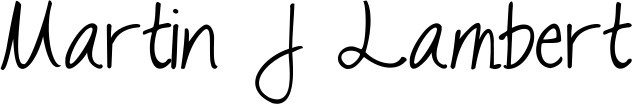
\includegraphics[width = 15em]{../img/my_signature.png}\\
  Martin John Lambert
\end{figure}

\addcontentsline{toc}{chapter}{Acknowledgements}
\chapter*{Acknowledgements}
I wish to sincerely thank all those who assisted me in achieving this monumental task.

\vspace{1em}
Firstly, I acknowledge the time, effort, knowledge, and (most importantly) patience given to me by my supervisors: Dr Drew Allen\footnote{\label{MQ}\ Macquarie University, Australia} for his foresight in experimental design and statistical finesse, and Dr Hendrik Poorter\footnote{\label{Julich}\ Forschungszentrum Jülich, Germany} for his expert knowledge on botanical experimentation and his academic guidance.

\vspace{1em}
I extend my thanks and appreciation to Dr Muhammad Masood\footnoteref{MQ} for his expert management of the Plant Growth Facility at Macquarie University where my glasshouse experiments were carried out. His diligence and assitance made what would have been a very stressful time a breeze.

\vspace{1em}
I also wish to thank Dr Ajay Narendra\footnoteref{MQ} and Dr Matthew Kosnik\footnoteref{MQ} for their management of the MRes programme at Macquarie University. Their knowledge of how to navigate through the tedious administrative tasks are greatly appreciated.

\vspace{1em}
Finally, but not at all least, I fondly extend my gratitute to two particular members of my fellow cohort who helped me in more ways than they know: Paige Lieurance\footnoteref{MQ} for her assistance with my glasshouse experiments, and Keira Chrystal\footnoteref{MQ} for her emotional support and level-headed accountability. And each again for their dear friendship.

\vspace{2em}
\begin{center}
  \Large
  \textbf{\textit{Ad maiorem Dei gloriam}}
\end{center}

\addcontentsline{toc}{chapter}{Thesis Abstract}
\chapter*{Thesis Abstract}
Lorem ipsum dolor sit amet, consectetur adipisicing elit, sed do eiusmod tempor incididunt ut labore et dolore magna aliqua. Ut enim ad minim veniam, quis nostrud exercitation ullamco laboris nisi ut aliquip ex ea commodo consequat. Duis aute irure dolor in reprehenderit in voluptate velit esse cillum dolore eu fugiat nulla pariatur. Excepteur sint occaecat cupidatat non proident, sunt in culpa qui officia deserunt mollit anim id est laborum.


\tableofcontents
\thispagestyle{empty}


\pagenumbering{arabic}
\begin{bibunit}

\addcontentsline{toc}{chapter}{Chapter 1: Literature Review}
\chapter*{Chapter 1\\ Literature Review}

\addcontentsline{toc}{section}{Abstract}
\section*{\begin{center}Abstract\end{center}}
Lorem ipsum dolor sit amet, consectetur adipisicing elit, sed do eiusmod tempor incididunt ut labore et dolore magna aliqua. Ut enim ad minim veniam, quis nostrud exercitation ullamco laboris nisi ut aliquip ex ea commodo consequat. Duis aute irure dolor in reprehenderit in voluptate velit esse cillum dolore eu fugiat nulla pariatur. Excepteur sint occaecat cupidatat non proident, sunt in culpa qui officia deserunt mollit anim id est laborum.

\vspace*{1.5cm}

\addcontentsline{toc}{section}{Introduction}
\section*{Introduction}
Lorem ipsum dolor sit amet, consectetur adipisicing elit, sed do eiusmod tempor incididunt ut labore et dolore magna aliqua \cite*{gufuExperimentalEvidenceThat2019}. Ut enim ad minim veniam, quis nostrud exercitation ullamco laboris nisi ut aliquip ex ea commodo consequat. Duis aute irure dolor in reprehenderit in voluptate velit esse cillum dolore eu fugiat nulla pariatur \cite*{hashemloianAlienExoticAzolla2009}. Excepteur sint occaecat cupidatat non proident, sunt in culpa qui officia deserunt mollit anim id est laborum. Lorem ipsum dolor sit amet, consectetur adipisicing elit, sed do eiusmod tempor incididunt ut labore et dolore magna aliqua. Ut enim ad minim veniam, quis nostrud exercitation ullamco laboris nisi ut aliquip ex ea commodo consequat. Duis aute irure dolor in reprehenderit in voluptate velit esse cillum dolore eu fugiat nulla pariatur \cite*{sadeghiReviewEcologicalFactors2013}. Excepteur sint occaecat cupidatat non proident, sunt in culpa qui officia deserunt mollit anim id est laborum.

\subsection*{subsection name}
Lorem ipsum dolor sit amet, consectetur adipisicing elit, sed do eiusmod tempor incididunt ut labore et dolore magna aliqua. Ut enim ad minim veniam, quis nostrud exercitation ullamco laboris nisi ut aliquip ex ea commodo consequat. Duis aute irure dolor in reprehenderit in voluptate velit esse cillum dolore eu fugiat nulla pariatur. Excepteur sint occaecat cupidatat non proident, sunt in culpa qui officia deserunt mollit anim id est laborum.

\addcontentsline{toc}{section}{References}
\putbib

\end{bibunit}


\begin{bibunit}

\addcontentsline{toc}{chapter}{Chapter 2: Materials and Methods}
\chapter*{Chapter 2\\ Materials and Methods}

\addcontentsline{toc}{section}{Abstract}
\section*{\begin{center}Abstract\end{center}}
Lorem ipsum dolor sit amet, consectetur adipisicing elit, sed do eiusmod tempor incididunt ut labore et dolore magna aliqua. Ut enim ad minim veniam, quis nostrud exercitation ullamco laboris nisi ut aliquip ex ea commodo consequat. Duis aute irure dolor in reprehenderit in voluptate velit esse cillum dolore eu fugiat nulla pariatur. Excepteur sint occaecat cupidatat non proident, sunt in culpa qui officia deserunt mollit anim id est laborum.

\vspace*{1.5cm}

\addcontentsline{toc}{section}{Introduction}
\section*{Introduction}
Lorem ipsum dolor sit amet, consectetur adipisicing elit, sed do eiusmod tempor incididunt ut labore et dolore magna aliqua. Ut enim ad minim veniam, quis nostrud exercitation ullamco laboris nisi ut aliquip ex ea commodo consequat. Duis aute irure dolor in reprehenderit in voluptate velit esse cillum dolore eu fugiat nulla pariatur. Excepteur sint occaecat cupidatat non proident, sunt in culpa qui officia deserunt mollit anim id est laborum \cite*{hashemloianAlienExoticAzolla2009, gufuGrowthReproductionFunctional2019}. Lorem ipsum dolor sit amet, consectetur adipisicing elit, sed do eiusmod tempor incididunt ut labore et dolore magna aliqua. Ut enim ad minim veniam, quis nostrud exercitation ullamco laboris nisi ut aliquip ex ea commodo consequat. Duis aute irure dolor in reprehenderit in voluptate velit esse cillum dolore eu fugiat nulla pariatur. Excepteur sint occaecat cupidatat non proident, sunt in culpa qui officia deserunt mollit anim id est laborum.

\section*{Initial Observations}
To determine the growth patterns of \textit{Azolla}, a small-scale observational experiment was conducted.

\vspace{1em}
\textit{Azolla} was harvested from the pond at the Plant Growth Facility at Macquarie University, Sydney, Australia (33.1923\textdegree S, 151.5749\textdegree E). Within that pond, three different, deliberately chosen locations were appointed to select a variety of \textit{Azolla} plants in different stages of maturity (Figure \ref{fig:MQ_pond}): a carpet at the edge of pond; a carpet in the middle of the pond; a low-density cluster in the middle of the pond. An additional 20L of pond water was extracted and passed through a coarse sieve to remove larger debris.

\begin{figure}[H]
  \centering
  \includegraphics[width = 35em]{img/pond.png}
  \caption{Pond at Macquarie University. A) A view of the pond. B) Carpet of \textit{Azolla} at the edge of the pond. C) Carpet of \textit{Azolla} in the middle of the pond. D) Low-density cluster of \textit{Azolla} in the middle of the pond.}
  \label{fig:MQ_pond}
\end{figure}

Non-BPA, UV resistant, food-grade 10L plastic tubs (internal dimensions approximately 346mm long x 242mm wide x 134mm deep, Appendix 1) were used to contain the treatments. Prior to use, the tubs were sprayed liberally with hydrogen peroxide (0.5\% w/w) then thoroughly rinsed with reverse osmosis (RO) water. Three tubs were each filled with 5L of the gathered pond water, 3 tubs were each filled with 5L of RO water. Five litres came to an average depth of 65mm in the centre of each tub.

\vspace{1em}
Seven fronds of \textit{Azolla} were selected by hand from the bucket in a hexagram pattern to alleviate selection bias (Figure \ref{fig:hexagram}). After these fronds were selected for a tub, the bucket’s contents were gently stirred using a flat wooden stick in a clockwise rotation for seven full revolutions to randomise the fronds’ locations for the next tub’s selection. Upon selection, each frond was inspected to ensure its maturity and root integrity (see Figure \ref{fig:frond_examples} for examples). Any fronds not found to be suitable were omitted. The 7 selected fronds were collectively placed onto the surface of the water at the centre of each tub.

\begin{figure}[H]
  \centering
  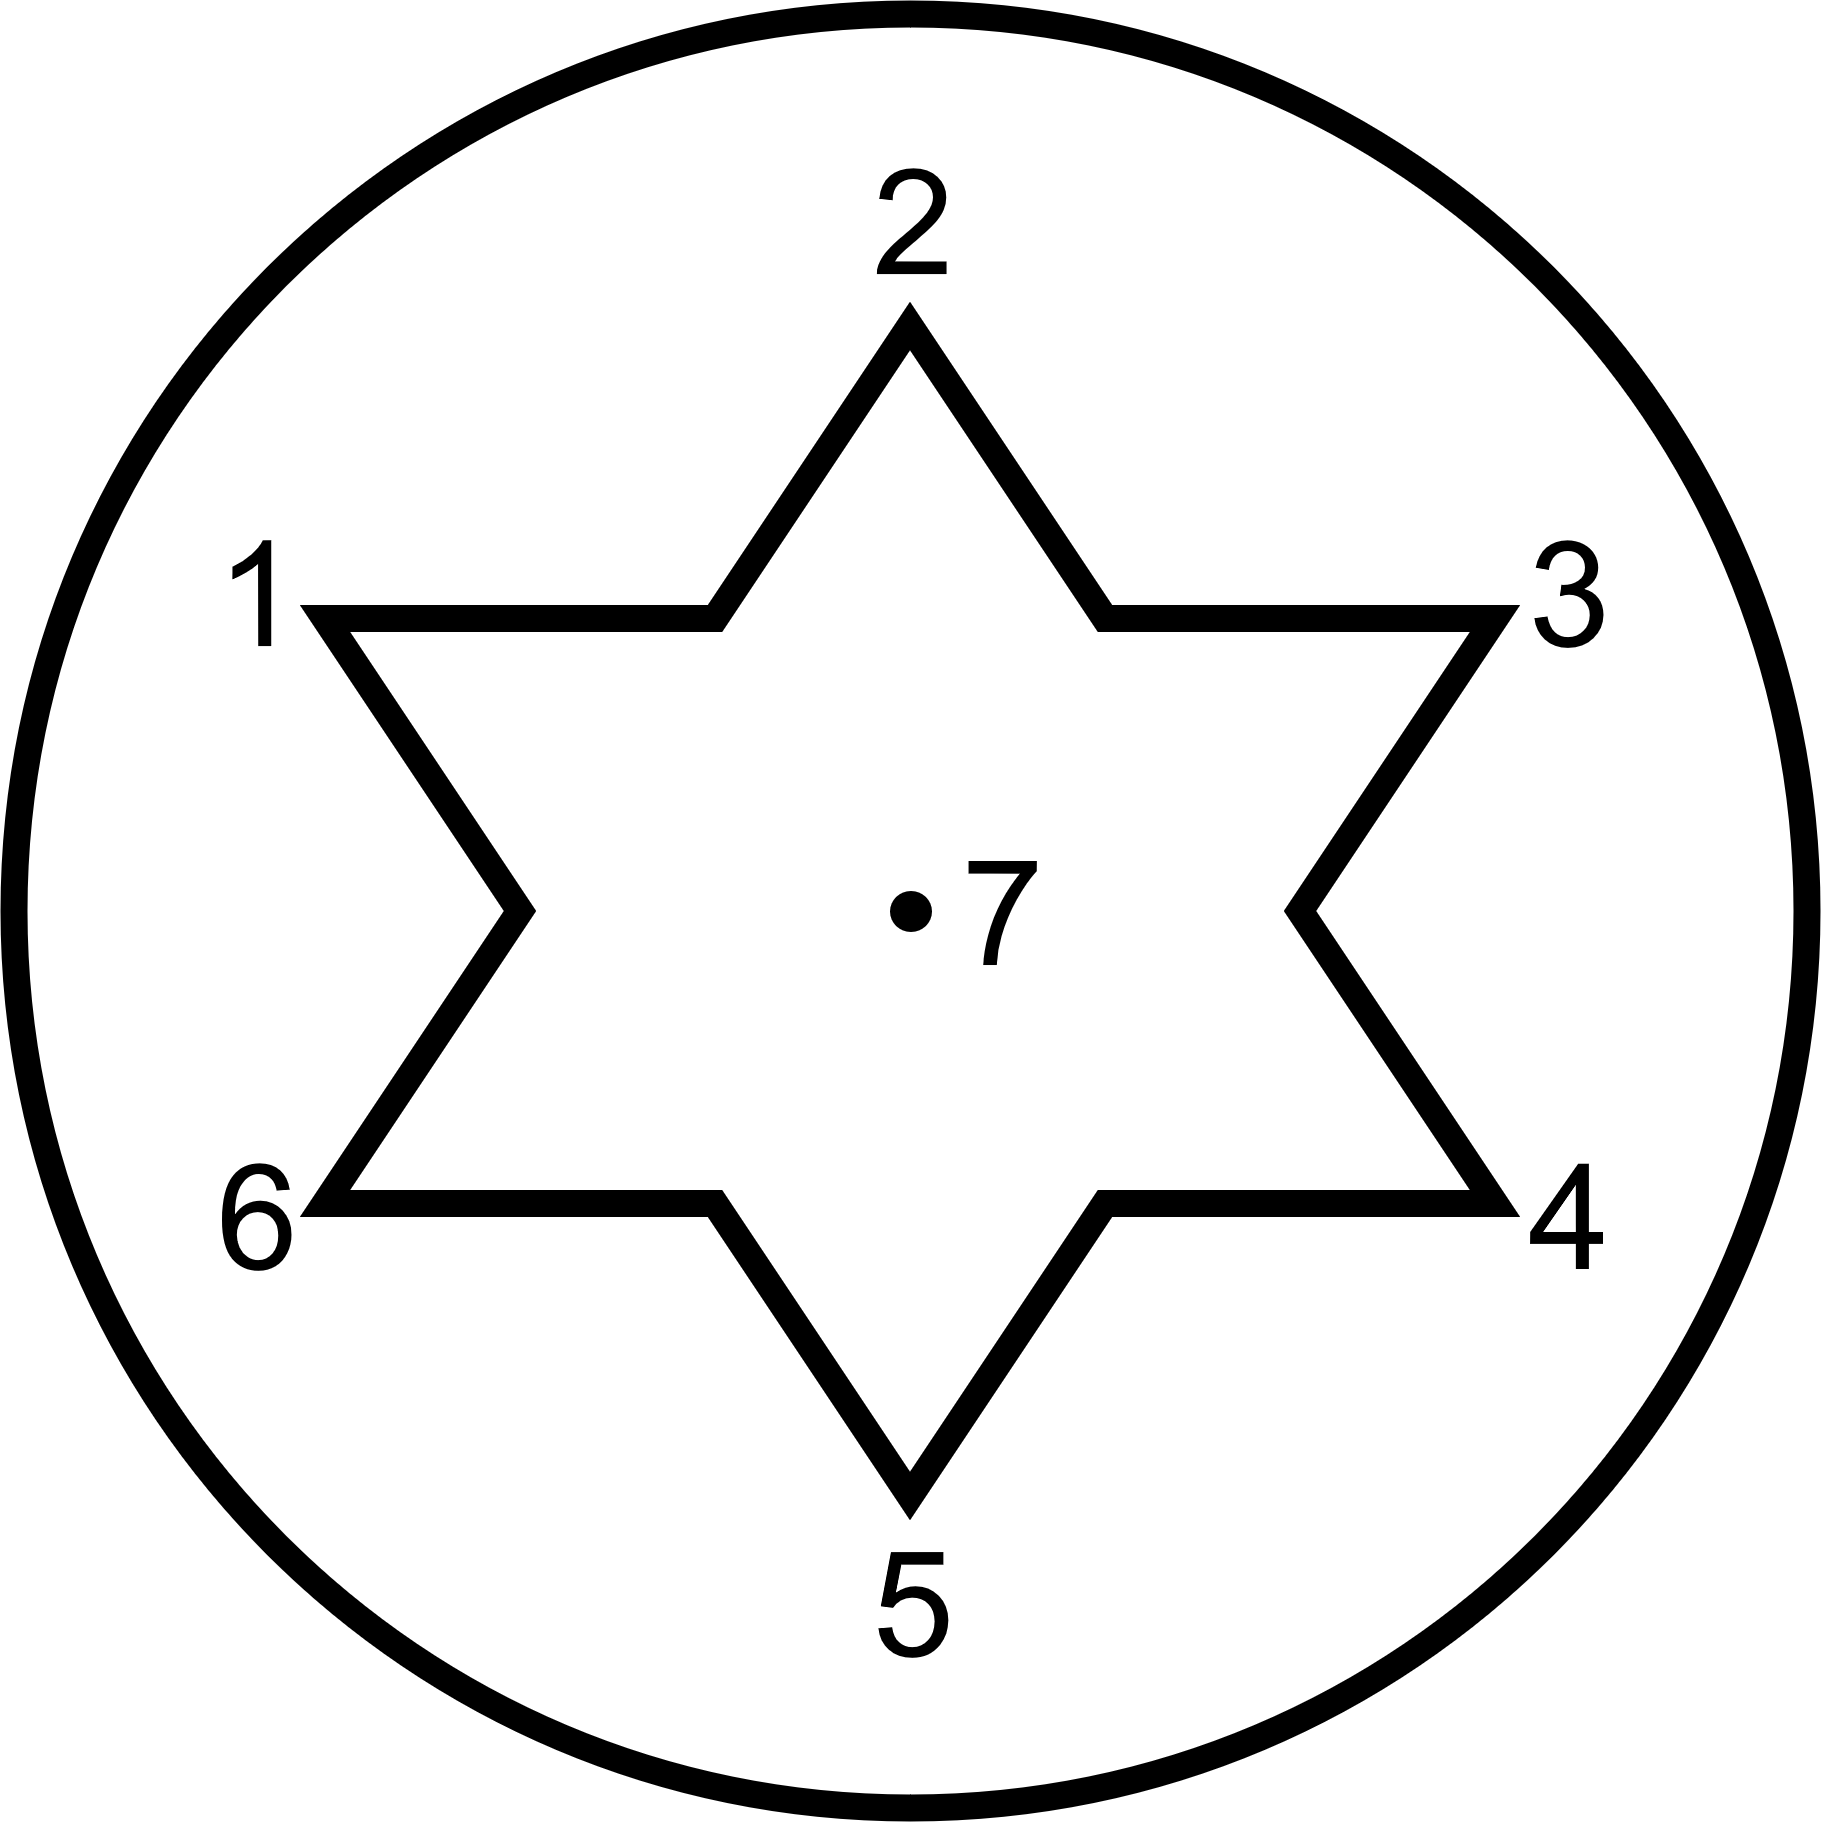
\includegraphics[width = 15em]{img/hexagram.png}
  \caption{Hexagram pattern. The 7 \textit{Azolla} fronds were selected from the edge of the bucket and at its centre by following the pattern laid out in this diagram.}
  \label{fig:hexagram}
\end{figure}

\begin{figure}[H]
  \centering
  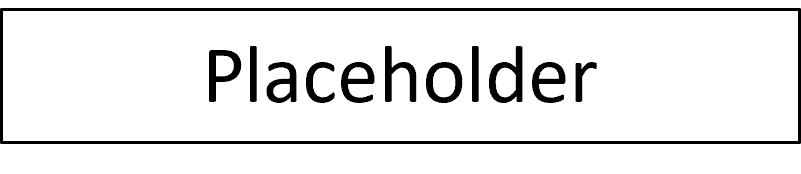
\includegraphics[width = 30em]{img/frond_examples.png}
  \caption{Examples of selected fronds. A) Mature and healthy frond (included). B) Immature frond (omitted). C) Damaged frond (omitted).}
  \label{fig:frond_examples}
\end{figure}

The tubs were temporarily placed in a line in random order in the middle of a glasshouse. This glasshouse was shared with another researcher who required the following environmental conditions: CO2 at 400ppm, ambient lighting, day temperature at 24-26\textdegree C and night temperature at 18-20\textdegree C for 12 hours each.

\vspace{1em}
After 5 days, 20mL of a commercial-grade liquid fertiliser was added to each tub (For chemical composition, see Appendix 2). The tubs’ arrangement was randomised to account for any within-glasshouse effects.

\vspace{1em}
Whenever the tubs were moved, care was taken to minimise any turbulence of the water that might break the surface tension and damage the fronds.


\addcontentsline{toc}{section}{References}
\putbib

\end{bibunit}


\begin{bibunit}

\addcontentsline{toc}{chapter}{Chapter 3: Results}
\chapter*{Chapter 3\\ Results}

\addcontentsline{toc}{section}{Abstract}
\section*{\begin{center}Abstract\end{center}}
Lorem ipsum dolor sit amet, consectetur adipisicing elit, sed do eiusmod tempor incididunt ut labore et dolore magna aliqua. Ut enim ad minim veniam, quis nostrud exercitation ullamco laboris nisi ut aliquip ex ea commodo consequat. Duis aute irure dolor in reprehenderit in voluptate velit esse cillum dolore eu fugiat nulla pariatur. Excepteur sint occaecat cupidatat non proident, sunt in culpa qui officia deserunt mollit anim id est laborum.

\vspace*{1.5cm}

\addcontentsline{toc}{section}{Introduction}
\section*{Introduction}
Lorem ipsum dolor sit amet, consectetur adipisicing elit, sed do eiusmod tempor incididunt ut labore et dolore magna aliqua. Ut enim ad minim veniam, quis nostrud exercitation ullamco laboris nisi ut aliquip ex ea commodo consequat. Duis aute irure dolor in reprehenderit in voluptate velit esse cillum dolore eu fugiat nulla pariatur \cite*{gufuGrowthReproductionFunctional2019}. Excepteur sint occaecat cupidatat non proident, sunt in culpa qui officia deserunt mollit anim id est laborum. Lorem ipsum dolor sit amet, consectetur adipisicing elit, sed do eiusmod tempor incididunt ut labore et dolore magna aliqua. Ut enim ad minim veniam, quis nostrud exercitation ullamco laboris nisi ut aliquip ex ea commodo consequat. Duis aute irure dolor in reprehenderit in voluptate velit esse cillum dolore eu fugiat nulla pariatur. Excepteur sint occaecat cupidatat non proident, sunt in culpa qui officia deserunt mollit anim id est laborum.

\subsection*{subsection name}
Lorem ipsum dolor sit amet, consectetur adipisicing elit, sed do eiusmod tempor incididunt ut labore et dolore magna aliqua. Ut enim ad minim veniam, quis nostrud exercitation ullamco laboris nisi ut aliquip ex ea commodo consequat. Duis aute irure dolor in reprehenderit in voluptate velit esse cillum dolore eu fugiat nulla pariatur. Excepteur sint occaecat cupidatat non proident, sunt in culpa qui officia deserunt mollit anim id est laborum.

\addcontentsline{toc}{section}{References}
\putbib

\end{bibunit}


\begin{bibunit}

\addcontentsline{toc}{chapter}{Chapter 4: Discussion}
\chapter*{Chapter 4\\ Discussion}

\addcontentsline{toc}{section}{Abstract}
\section*{\begin{center}Abstract\end{center}}
Lorem ipsum dolor sit amet, consectetur adipisicing elit, sed do eiusmod tempor incididunt ut labore et dolore magna aliqua. Ut enim ad minim veniam, quis nostrud exercitation ullamco laboris nisi ut aliquip ex ea commodo consequat. Duis aute irure dolor in reprehenderit in voluptate velit esse cillum dolore eu fugiat nulla pariatur. Excepteur sint occaecat cupidatat non proident, sunt in culpa qui officia deserunt mollit anim id est laborum.

\vspace*{1.5cm}

\addcontentsline{toc}{section}{Introduction}
\section*{Introduction}
Lorem ipsum dolor sit amet, consectetur adipisicing elit, sed do eiusmod tempor incididunt ut labore et dolore magna aliqua. Ut enim ad minim veniam, quis nostrud exercitation ullamco laboris nisi ut aliquip ex ea commodo consequat. Duis aute irure dolor in reprehenderit in voluptate velit esse cillum dolore eu fugiat nulla pariatur \cite*{hashemloianAlienExoticAzolla2009}. Excepteur sint occaecat cupidatat non proident, sunt in culpa qui officia deserunt mollit anim id est laborum. Lorem ipsum dolor sit amet, consectetur adipisicing elit, sed do eiusmod tempor incididunt ut labore et dolore magna aliqua. Ut enim ad minim veniam, quis nostrud exercitation ullamco laboris nisi ut aliquip ex ea commodo consequat. Duis aute irure dolor in reprehenderit in voluptate velit esse cillum dolore eu fugiat nulla pariatur \cite*{gufuExperimentalEvidenceThat2019, hashemloianAlienExoticAzolla2009}. Excepteur sint occaecat cupidatat non proident, sunt in culpa qui officia deserunt mollit anim id est laborum.

\subsection*{subsection name}
Lorem ipsum dolor sit amet, consectetur adipisicing elit, sed do eiusmod tempor incididunt ut labore et dolore magna aliqua \cite*{gufuGrowthReproductionFunctional2019}. Ut enim ad minim veniam, quis nostrud exercitation ullamco laboris nisi ut aliquip ex ea commodo consequat. Duis aute irure dolor in reprehenderit in voluptate velit esse cillum dolore eu fugiat nulla pariatur. Excepteur sint occaecat cupidatat non proident, sunt in culpa qui officia deserunt mollit anim id est laborum.

\addcontentsline{toc}{section}{References}
\putbib

\end{bibunit}


\include{tex/appendix.tex}

\addcontentsline{toc}{section}{Thesis References}


\end{document}
